\documentclass[12pt,a4paper]{article}
\renewcommand{\baselinestretch}{1.5}
\usepackage{placeins}
\usepackage[T1]{fontenc}
\usepackage[utf8]{inputenc}
\usepackage{amsmath}
\usepackage{amsfonts}
\usepackage{amssymb}
\usepackage{algorithm}
\usepackage{algpseudocode}
\usepackage{graphicx}
\usepackage{geometry}
\usepackage{float}
\usepackage{caption}
\usepackage{subcaption}
\usepackage{booktabs}
\usepackage{array}
\usepackage{longtable}
\usepackage{xcolor}
\usepackage{listings}
\usepackage{tikz}
\usetikzlibrary{positioning,shapes.geometric,arrows.meta}
\usepackage{pgfplots}
\pgfplotsset{compat=1.18}
\usepackage{bm}
\usepackage[hyphens]{url}
\usepackage{hyperref}
\hypersetup{colorlinks=true,linkcolor=black,citecolor=black,urlcolor=blue}

\usepackage{titlesec}
\setcounter{secnumdepth}{4}
\setcounter{tocdepth}{3}

\geometry{left=2cm,right=2cm,top=1.5cm,bottom=2cm}
\setlength{\footskip}{20pt}
\graphicspath{{./}}
\setlength{\emergencystretch}{2em}

\lstset{
    basicstyle=\ttfamily\small,
    breaklines=true,
    frame=single,
    numbers=left,
    numberstyle=\tiny\color{gray},
    captionpos=b,
    language=C,
    tabsize=4,
    showstringspaces=false,
    commentstyle=\color{gray!70},
    keywordstyle=\color{blue!80}\bfseries,
    stringstyle=\color{red!70},
    xleftmargin=1.5em,
    framexleftmargin=1.5em,
}

%% ================================================================
\begin{document}

\thispagestyle{empty}
\begin{center}
	{\Large \bf Parallel Document Similarity Search\\}
	
	\vspace*{0.5cm}
	{\large\textit{A Project Report Submitted in Partial Fulfilment of the Requirements for}\\}
	{\large\textbf{Parallel and Distributed Computing (UCS645)}} \\

	{\large \textit{By\\}}
	\textbf{\begin{table}[h!]
\label{tab:students}
\centering
\begin{tabular}{ccc}
\textbf{Sr} & \textbf{Name}         & \textbf{Roll No}   \\
1           & Aarav Dudeja          & 102303179          \\
2           & Arunav Joshi          & 102303166          \\
3           & Kanav Mahajan         & 102303102          \\
4           & Vaani Prashar         & 102303159          \\
\end{tabular}
\end{table}}

	\begin{center}
                {\large \textit{Under the guidance of}}\\
				\textbf{{\large Dr. Saif Nalband}}\\
				{\large (Assistant Professor, DCSE)}\\
	\end{center}
	\ \\ \ \\
\begin{figure}[h]
\centering

\includegraphics[width=70mm, height=40mm]{tietlogo.jpg}
\label{fig:tietlogo}
\end{figure}

	\vspace*{0.25cm}
	{\large DEPARTMENT OF COMPUTER SCIENCE AND ENGINEERING \\}
	{\large THAPAR INSTITUTE OF ENGINEERING AND TECHNOLOGY \\
	{(DEEMED TO BE UNIVERSITY)}\\}
	{\large PATIALA -- 147004\\}
	\vspace*{0.3cm}
	\textbf{{\large MAY, 2025}}
	
\end{center}

\newpage

\pagenumbering{gobble}

\renewcommand*\contentsname{Table of Contents}
\tableofcontents
\newpage
\listoffigures
\newpage
\listoftables
\newpage
\pagenumbering{arabic}

%% ================================================================
\clearpage
\section{Introduction}

\subsection{Background}

Document similarity search is the problem of finding, from a large
collection of documents, those that are most similar to a given query.
It is central to many practical applications: search engines, plagiarism
detectors, recommendation systems, and duplicate record finders all
depend on fast and accurate similarity computation \cite{manning2008}.

Representing documents as fixed-length numerical feature vectors reduces
the problem to computing a distance or angle in vector space. The
challenge is scale -- comparing a query against tens of thousands of
documents on a single processor becomes a bottleneck when the feature
dimension or corpus size grows.

Parallel computing addresses this by dividing the corpus across multiple
processors and letting each processor handle its own portion
independently. The Message Passing Interface (MPI) coordinates this
across separate processes, while OpenMP exploits the multiple cores
within a single processor using shared-memory threads \cite{gropp1999mpi}.
Combining the two -- a \textit{hybrid} parallel model -- makes use of
both levels simultaneously and is the standard approach in
high-performance computing.

This project implements a hybrid MPI+OpenMP parallel document similarity
search system, evaluates its performance on a dataset of 10,000
documents, and analyses the results using Amdahl's Law.

\subsection{Problem Statement}

A corpus $\mathcal{D} = \{\mathbf{d}_1, \ldots, \mathbf{d}_n\}$ of $n$
documents is given, where each document $\mathbf{d}_i \in \mathbb{Z}^m$
is represented as an integer feature vector of length $m$. Given a query
$\mathbf{q} \in \mathbb{Z}^m$, the task is to identify the $k$ most
similar documents to $\mathbf{q}$ according to a chosen similarity
function $S$:
\begin{equation}
    \mathcal{T}_k = \underset{\mathcal{S} \subseteq \mathcal{D},\,
    |\mathcal{S}|=k}{\arg\max}
    \sum_{\mathbf{d} \in \mathcal{S}} S(\mathbf{q}, \mathbf{d})
\end{equation}

Total execution time is split into four measurable phases:
\begin{equation}
    T_{\text{total}} = T_{\text{I/O}} + T_{\text{scatter}} +
    T_{\text{compute}} + T_{\text{gather}}
\end{equation}

The parallel system targets $T_{\text{compute}}$ for reduction while
minimising overhead in the other three phases.

%% ================================================================
\clearpage
\section{Literature Review}

Table~\ref{tab:litreview} summarises the key references surveyed for
this project. The works span information retrieval, GPU-based similarity
search, graph-based approximate methods, and hybrid parallel programming.

\begin{longtable}{|c|p{3.2cm}|p{4.0cm}|p{6.8cm}|}
\caption{Summary of Literature Review}
\label{tab:litreview}\\
\hline
\textbf{Sr.} & \textbf{Reference} & \textbf{Technique} & \textbf{Contribution and Relevance} \\
\hline
\endfirsthead
\hline
\textbf{Sr.} & \textbf{Reference} & \textbf{Technique} & \textbf{Contribution and Relevance} \\
\hline
\endhead
\hline
\endfoot

1 &
Manning et al.\ (2008), \textit{Introduction to Information Retrieval},
Cambridge University Press &
TF-IDF weighting, cosine similarity, vector space model &
Defines the vector-space document representation and similarity metrics
used in this project. Standard reference for IR \cite{manning2008}. \\
\hline

2 &
Gropp, Lusk, Skjellum (1999), \textit{Using MPI}, MIT Press &
MPI point-to-point messaging, collective operations &
Definitive MPI programming reference. Basis for all inter-process
communication in the system, particularly \texttt{MPI\_Scatterv} and
\texttt{MPI\_Gather} \cite{gropp1999mpi}. \\
\hline

3 &
Johnson, Douze, Jegou (2021), \textit{IEEE Trans.\ Big Data} &
GPU $k$-selection via WarpSelect, product quantisation &
Achieves 8.5$\times$ speedup over prior GPU state-of-the-art for
nearest-neighbour search at billion scale. Motivates using a min-heap
as the CPU-side $k$-selection strategy \cite{johnson2021faiss}. \\
\hline

4 &
Douze et al.\ (2024), \textit{arXiv:2401.08281} &
IVF, HNSW, and PQ indices; unified FAISS library &
Industry-standard open-source library for large-scale similarity search.
Confirms that exact brute-force search remains viable when recall must
be 100\% \cite{douze2024faiss}. \\
\hline

5 &
Malkov \& Yashunin (2020), \textit{IEEE TPAMI} &
Hierarchical Navigable Small World (HNSW) proximity graphs &
Delivers sub-linear query time with high recall; now the backbone of
most production vector databases. Relevant as a future alternative to
brute-force search \cite{malkov2020hnsw}. \\
\hline

6 &
Aumuller, Bernhardsson, Faithfull (2020), \textit{Information Systems} &
Standardised recall-vs-time benchmarks for ANN algorithms &
Shows that no single approximate method dominates across all datasets.
Justifies the exact search approach when result correctness is
required \cite{aumuller2020ann}. \\
\hline

7 &
Lu et al.\ (2023), \textit{Frontiers in Earth Science} &
Hybrid MPI+OpenMP for scientific computing on CPU clusters &
Demonstrates that hybrid parallelism reduces memory replication
compared to pure MPI on multi-core nodes, directly motivating the
two-level parallel design used here \cite{lu2023hybrid}. \\
\hline

8 &
Velarde Martinez (2022), \textit{Applied Sciences} &
Comparative study of hybrid OpenMP+MPI versus pure MPI &
Reports up to 40\% runtime reduction using hybrid programming over
pure MPI for data-parallel workloads. Confirms that the benefit
depends on dataset size \cite{velarde2022hybrid}. \\
\hline

9 &
Thakur, Rabenseifner, Gropp (2005), \textit{IJHPCA} &
Optimised MPI collective algorithms using binomial trees &
Reduces collective communication latency by up to 62\% over
point-to-point loops. Justifies replacing a sequential scatter loop
with \texttt{MPI\_Scatterv} \cite{thakur2005mpi}. \\
\hline
\end{longtable}

Taken together, the literature points to three concrete design
decisions. The heap-based $k$-selection from Johnson et al.\
\cite{johnson2021faiss} and FAISS \cite{douze2024faiss} is adopted as
the top-$k$ algorithm on each MPI rank. The hybrid parallelism findings
of Lu et al.\ \cite{lu2023hybrid} and Velarde Martinez
\cite{velarde2022hybrid} motivate combining MPI with OpenMP threads.
Thakur et al.\ \cite{thakur2005mpi} provide the theoretical basis for
preferring \texttt{MPI\_Scatterv} over individual send calls.

%% ================================================================
\clearpage
\section{Research Gaps}

The following gaps were identified from the literature and addressed in
this project.

\textbf{Single-level parallelism.} Most CPU-based MPI implementations
assign one thread per rank, leaving remaining cores on the same machine
idle. The hybrid design activates all cores through OpenMP threads within
each rank.

\textbf{Inefficient top-$k$ selection.} Sorting all local documents
takes $O(n \log n)$ time and $O(n)$ memory even when only $k \ll n$
results are needed. A min-heap reduces this to $O(n \log k)$ with
$O(k)$ memory.

\textbf{Suboptimal scatter communication.} Sending document partitions
one by one using \texttt{MPI\_Send} incurs $O(P)$ sequential latencies.
A single \texttt{MPI\_Scatterv} call completes the same operation in
$O(\log P)$ via the MPI runtime's binomial tree.

\textbf{Gather correctness bug.} When a rank holds fewer than $k$
documents, passing a variable send count to \texttt{MPI\_Gather} causes
a buffer size mismatch and corrupts memory. Padding each rank's output
to a uniform $k$ entries with sentinel values eliminates this.

\textbf{Manhattan distance bug.} Using \texttt{abs()} on a
\texttt{double} value silently truncates the fractional part before
taking the absolute value, producing incorrect distances. The fix is to
use \texttt{fabs()} from \texttt{<math.h>}.

\textbf{Single metric.} Most prior implementations support only cosine
similarity. This system exposes four metrics through a common interface
so the user can choose at runtime.

%% ================================================================
\clearpage
\section{Problem Formulation}

\subsection{Similarity Metrics}

Four similarity functions are supported. Euclidean and Manhattan
distances are negated so that a higher score always means greater
similarity, consistent with the power and cosine formulations.

\begin{enumerate}
\item \textbf{Power-based similarity}:
\begin{equation}
    S_{\text{power}}(\mathbf{q},\mathbf{d}_i)
    = \sum_{j=1}^{m} d_{i,j}^{\,q_j}
\end{equation}

\item \textbf{Cosine similarity}:
\begin{equation}
    S_{\text{cosine}}(\mathbf{q},\mathbf{d}_i)
    = \frac{\mathbf{q}\cdot\mathbf{d}_i}
           {\|\mathbf{q}\|_2\,\|\mathbf{d}_i\|_2}
\end{equation}

\item \textbf{Euclidean distance} (negated):
\begin{equation}
    S_{\text{euclidean}}(\mathbf{q},\mathbf{d}_i)
    = -\sqrt{\sum_{j=1}^{m}(q_j-d_{i,j})^2}
\end{equation}

\item \textbf{Manhattan distance} (negated):
\begin{equation}
    S_{\text{manhattan}}(\mathbf{q},\mathbf{d}_i)
    = -\sum_{j=1}^{m}|q_j-d_{i,j}|
\end{equation}
\end{enumerate}

\subsection{Parallel Work Distribution}

With $P$ MPI ranks, the corpus is split into $P$ contiguous blocks.
Rank $r$ receives:
\begin{equation}
    |\mathcal{D}_r|
    = \left\lfloor\frac{n}{P}\right\rfloor
    + \begin{cases}1 & r < (n \bmod P)\\0 & \text{otherwise}\end{cases}
\end{equation}

Load imbalance between any two ranks is at most one document. Each rank
independently computes its local top-$k$ list, and rank 0 merges all
lists to produce the final answer:
\begin{equation}
    \mathcal{T}_k
    = \mathrm{TopK}\!\left(\bigcup_{r=0}^{P-1}\mathcal{T}_k^{(r)}\right)
\end{equation}

With $T$ OpenMP threads per rank, $P \times T$ hardware threads are
active during the computation phase.

%% ================================================================
\clearpage
\section{Objectives}

The objectives of this project are as follows.

\begin{enumerate}
\item Implement a hybrid MPI+OpenMP parallel document similarity search
      system that correctly exploits both distributed-memory and
      shared-memory parallelism.

\item Replace the sequential document scatter loop with
      \texttt{MPI\_Scatterv} and implement sentinel-padded
      \texttt{MPI\_Gather} to ensure both efficiency and correctness
      in inter-process communication.

\item Implement $O(n\log k)$ top-$k$ selection using a min-heap,
      replacing the $O(n\log n)$ full sort used in the baseline
      \cite{cormen2022algorithms}.

\item Support four similarity metrics (Power, Cosine, Euclidean,
      Manhattan) selectable at runtime without recompilation.

\item Profile execution in four phases (I/O, scatter, compute, gather)
      using \texttt{MPI\_Wtime} and analyse scalability using
      Amdahl's Law.

\item Verify that the top-$k$ output is identical across all tested
      rank and thread configurations.
\end{enumerate}

%% ================================================================
\clearpage
\section{Methodology}

\subsection{System Architecture}

The program follows a master--worker structure with two levels of
parallelism. Figure~\ref{fig:arch} shows the complete data flow.
Rank 0 reads all input files and broadcasts the query vector and
metadata to every rank using \texttt{MPI\_Bcast}. Document blocks are
distributed via a single \texttt{MPI\_Scatterv} call. Each rank then
runs its OpenMP-parallelised scoring loop and builds a local min-heap
of the top-$k$ candidates. Finally, all ranks send their padded top-$k$
arrays to rank 0 via \texttt{MPI\_Gather}, and rank 0 performs the
global merge.

\begin{figure}[!htbp]
\centering
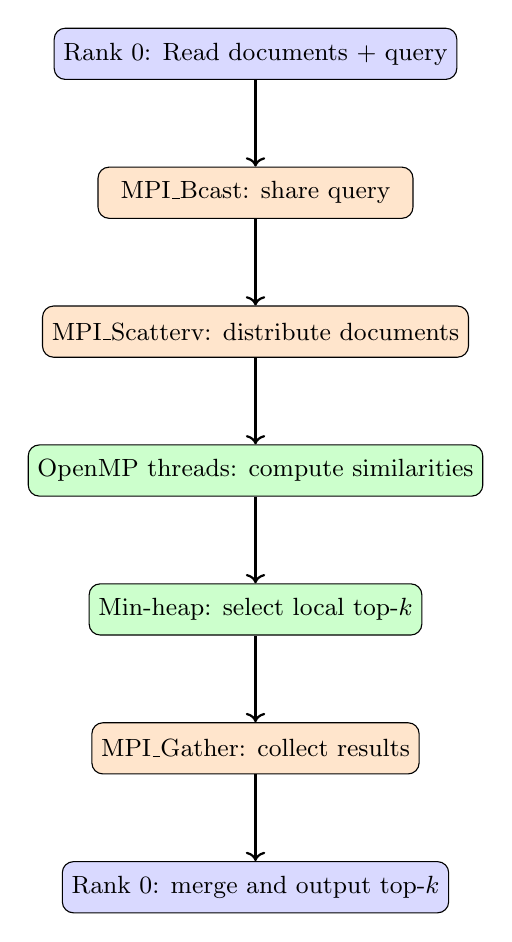
\begin{tikzpicture}[
    node distance=1.1cm,
    box/.style={rectangle,draw,rounded corners,
                minimum width=4.0cm,minimum height=0.65cm,
                font=\small,align=center},
    arr/.style={->,thick}]
\node[box,fill=blue!15]   (io)    {Rank 0: Read documents + query};
\node[box,fill=orange!20,below=of io]   (bcast){MPI\_Bcast: share query};
\node[box,fill=orange!20,below=of bcast](scat) {MPI\_Scatterv: distribute documents};
\node[box,fill=green!20, below=of scat] (omp)  {OpenMP threads: compute similarities};
\node[box,fill=green!20, below=of omp]  (heap) {Min-heap: select local top-$k$};
\node[box,fill=orange!20,below=of heap] (gath) {MPI\_Gather: collect results};
\node[box,fill=blue!15,  below=of gath] (merge){Rank 0: merge and output top-$k$};
\draw[arr](io)--(bcast);\draw[arr](bcast)--(scat);
\draw[arr](scat)--(omp);\draw[arr](omp)--(heap);
\draw[arr](heap)--(gath);\draw[arr](gath)--(merge);
\end{tikzpicture}
\caption{System data flow. Blue = rank 0 only; orange = MPI collective
         operations ($O(\log P)$ complexity); green = all ranks with
         OpenMP thread-level parallelism.}
\label{fig:arch}
\end{figure}

\subsection{Top-K Selection with Min-Heap}

\begin{algorithm}[H]
\caption{Local Top-K Selection (executed on every MPI rank)}
\begin{algorithmic}[1]
\State \textbf{Input:} document partition $\mathcal{D}_r$, query
       $\mathbf{q}$, integer $k$
\State \textbf{Output:} sorted top-$k$ result array
\Comment{Phase A -- parallel (OpenMP)}
\For{each $\mathbf{d}_i \in \mathcal{D}_r$ \textbf{in parallel}}
    \State $\mathrm{scores}[i] \gets S(\mathbf{q},\mathbf{d}_i)$
\EndFor
\Comment{Phase B -- sequential heap}
\State $H \gets$ empty min-heap of capacity $k$
\For{$i=0$ to $|\mathcal{D}_r|-1$}
    \State \Call{Insert}{$H$, id$[i]$, scores$[i]$}
\EndFor
\State \Return sorted contents of $H$ in descending order
\end{algorithmic}
\end{algorithm}

The two-phase structure is important. The similarity computation
(Phase A) is the expensive part and runs in parallel across all $T$
OpenMP threads. Heap maintenance (Phase B) is sequential but inexpensive:
each insertion costs $O(\log k)$, giving a total per-rank complexity of
$O((n/P)\log k)$ compared to $O((n/P)\log(n/P))$ for a full sort
\cite{cormen2022algorithms}.

\subsection{Global Result Collection (KReduce)}

\begin{algorithm}[H]
\caption{KReduce: Collecting Global Top-K}
\begin{algorithmic}[1]
\State Each rank pads its local top-$k$ array to exactly $k$ entries,
       filling empty slots with sentinels (id~$= -1$, score~$= -\infty$)
\State \Call{MPI\_Gather}{padded array from all ranks to rank 0}
\If{rank $= 0$}
    \State Remove all sentinel entries
    \State Sort remaining entries by score (descending)
    \State Return first $k$ entries as the global top-$k$
\EndIf
\end{algorithmic}
\end{algorithm}

Without the padding step, any rank that holds fewer than $k$ documents
would send a smaller buffer, causing \texttt{MPI\_Gather} to read
beyond the end of receive buffers on rank 0 -- a classic memory
corruption bug.

\subsection{OpenMP Parallelisation}

Within each MPI rank, the similarity loop uses a dynamic schedule to
balance work across threads:

\begin{lstlisting}[caption={OpenMP parallel loop for similarity scoring}]
#pragma omp parallel for schedule(dynamic, 64) default(none) \
    shared(local_documents, query_arr, scores,
           local_count, dict_size, metric)
for (int i = 0; i < local_count; i++) {
    scores[i] = computeSimilarity(dict_size,
                    &local_documents[i * dict_size],
                    query_arr, metric);
}
\end{lstlisting}

\texttt{schedule(dynamic,64)} assigns chunks of 64 documents to
whichever thread is next available, which helps keep all threads busy
when computation costs vary across documents \cite{openmp51}.

\subsection{Core Data Structures}

\begin{lstlisting}[caption={Core type definitions from utils.h}]
typedef struct { int id; double score; } DocScore;

typedef struct {
    DocScore *heap;
    int       capacity;   /* always equal to k */
    int       size;
} MinHeap;

typedef enum {
    SIMILARITY_POWER, SIMILARITY_COSINE,
    SIMILARITY_EUCLIDEAN, SIMILARITY_MANHATTAN
} SimilarityMetric;
\end{lstlisting}

%% ================================================================
\clearpage
\section{Dataset}

\begin{table}[!htbp]
\centering
\small
\caption{Datasets Used for Experiments}
\label{tab:datasets}
\renewcommand{\arraystretch}{1.3}
\begin{tabular}{|l|p{4.5cm}|c|c|c|}
\hline
\textbf{Name} & \textbf{Purpose} &
\textbf{Size} & \textbf{Documents} & \textbf{Features ($m$)} \\
\hline
Small  & Correctness verification &
$\approx$3~KB   & 100    & 10 \\
\hline
Medium & All timing and scaling experiments &
$\approx$2.8~MB & 10,000 & 10 \\
\hline
Large  & Stress test with high-dimensional vectors &
$\approx$29~MB  & 10,000 & 100 \\
\hline
\end{tabular}
\end{table}

All datasets were generated using the provided \texttt{generate\_data.py}
script with seed 42, ensuring reproducibility. Each line in the document
file follows the format:
\begin{center}
\texttt{<id>: <f\textsubscript{1}> <f\textsubscript{2}> \ldots\ <f\textsubscript{m}>}
\end{center}
Custom datasets of any size can be generated by adjusting the
\texttt{--docs} and \texttt{--features} arguments to the script.

%% ================================================================
\clearpage
\section{Results and Discussion}

\subsection{Experimental Setup}

Experiments were conducted on a WSL2 (Windows Subsystem for Linux 2)
environment running on a multi-core Intel CPU. The toolchain was
\texttt{mpicc} (GCC) with flags \texttt{-Wall -O3 -std=c99 -fopenmp},
OpenMPI, and GCC \texttt{libgomp}. All scaling experiments used the
Medium dataset (10,000 documents, $m=10$, $k=10$). MPI ranks of 1, 2,
4, and 6 were tested; the machine does not support more than 6 reliable
ranks. Each experiment was run after a fresh dataset generation with
seed 42.

%% ================================================================
\subsection{MPI Strong Scaling}
\label{sec:mpi}

Table~\ref{tab:scaling} reports per-phase timings across MPI rank counts
with OpenMP threads fixed at 1. Table~\ref{tab:speedup} derives the
computation-phase speedup and parallel efficiency.

\begin{table}[!htbp]
\centering
\small
\caption{Raw Timings: MPI Strong Scaling (Power metric, OMP = 1)}
\label{tab:scaling}
\renewcommand{\arraystretch}{1.3}
\begin{tabular}{|c|c|c|c|c|c|}
\hline
\textbf{Ranks} & \textbf{I/O (s)} & \textbf{Scatter (s)} &
\textbf{Compute (s)} & \textbf{Gather (s)} & \textbf{Total (s)} \\
\hline
1 & 0.009724 & 0.000375 & 0.002113 & 0.000006 & 0.012282 \\
2 & 0.016951 & 0.001948 & 0.003627 & 0.001225 & 0.023967 \\
4 & 0.012760 & 0.001506 & 0.001771 & 0.000032 & 0.016153 \\
6 & 0.013809 & 0.001273 & 0.000613 & 0.000464 & 0.016265 \\
\hline
\end{tabular}
\end{table}

\begin{table}[!htbp]
\centering
\small
\caption{Computation-Phase Speedup and Parallel Efficiency}
\label{tab:speedup}
\renewcommand{\arraystretch}{1.3}
\begin{tabular}{|c|c|c|c|}
\hline
\textbf{MPI Ranks} & \textbf{Compute (s)} &
\textbf{Speedup} & \textbf{Efficiency} \\
\hline
1 (baseline) & 0.002113 & 1.00$\times$ & 100.0\% \\
2            & 0.003627 & 0.58$\times$ &  29.1\% \\
4            & 0.001771 & 1.19$\times$ &  29.8\% \\
6            & 0.000613 & 3.45$\times$ &  57.4\% \\
\hline
\end{tabular}
\end{table}

\begin{figure}[!htbp]
\centering
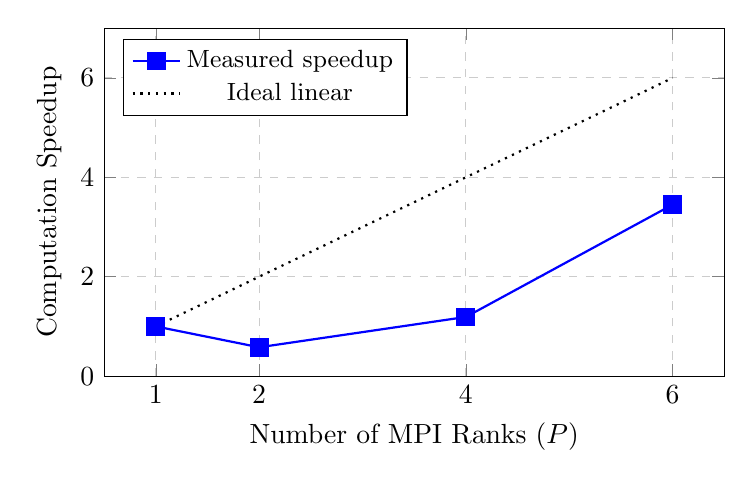
\begin{tikzpicture}
\begin{axis}[
    width=0.78\textwidth, height=6cm,
    xlabel={Number of MPI Ranks ($P$)},
    ylabel={Computation Speedup},
    xtick={1,2,4,6}, xticklabels={1,2,4,6},
    legend pos=north west, legend style={font=\small},
    grid=major, grid style={dashed,gray!40},
    ymin=0, ymax=7,
]
\addplot[blue,mark=square*,thick,mark size=3pt]
    coordinates {(1,1.00)(2,0.58)(4,1.19)(6,3.45)};
\addlegendentry{Measured speedup}
\addplot[black,dotted,thick]
    coordinates {(1,1)(2,2)(4,4)(6,6)};
\addlegendentry{Ideal linear}
\end{axis}
\end{tikzpicture}
\caption{Computation-phase speedup vs MPI rank count. The dip at $P=2$
         is a WSL2 process-launch artefact discussed in
         Section~\ref{sec:disc}. At $P=6$ the speedup reaches
         3.45$\times$.}
\label{fig:speedup}
\end{figure}

\begin{figure}[!htbp]
\centering
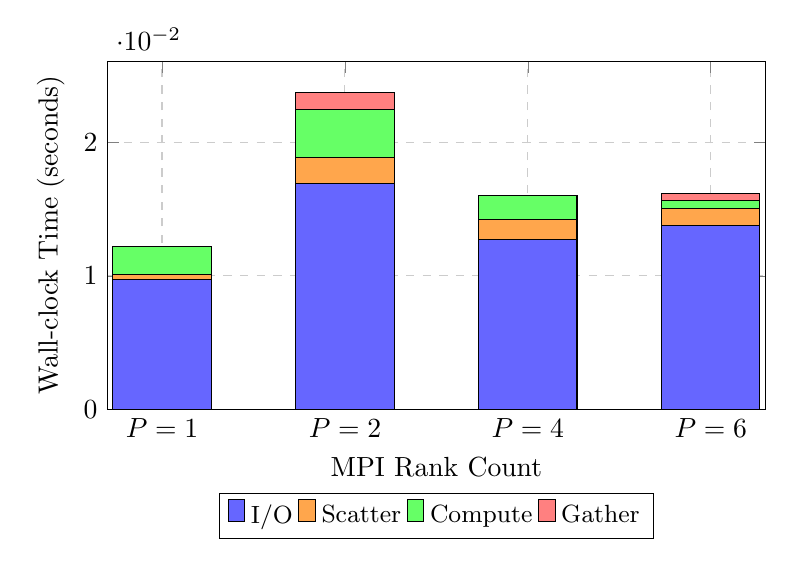
\begin{tikzpicture}
\begin{axis}[
    ybar stacked,
    width=0.82\textwidth, height=6cm,
    symbolic x coords={$P=1$,$P=2$,$P=4$,$P=6$},
    xtick=data,
    xlabel={MPI Rank Count},
    ylabel={Wall-clock Time (seconds)},
    legend style={at={(0.5,-0.24)},anchor=north,legend columns=4,font=\small},
    bar width=1.25cm, ymin=0,
    grid=major, grid style={dashed,gray!40},
]
\addplot[fill=blue!60]
    coordinates {($P=1$,0.009724)($P=2$,0.016951)($P=4$,0.012760)($P=6$,0.013809)};
\addlegendentry{I/O}
\addplot[fill=orange!70]
    coordinates {($P=1$,0.000375)($P=2$,0.001948)($P=4$,0.001506)($P=6$,0.001273)};
\addlegendentry{Scatter}
\addplot[fill=green!60]
    coordinates {($P=1$,0.002113)($P=2$,0.003627)($P=4$,0.001771)($P=6$,0.000613)};
\addlegendentry{Compute}
\addplot[fill=red!50]
    coordinates {($P=1$,0.000006)($P=2$,0.001225)($P=4$,0.000032)($P=6$,0.000464)};
\addlegendentry{Gather}
\end{axis}
\end{tikzpicture}
\caption{Stacked phase breakdown across all rank counts (Power metric,
         OMP = 1). I/O (blue) dominates every run and does not decrease
         with more ranks. Compute (green) shrinks clearly from $P=1$
         to $P=6$.}
\label{fig:stacked}
\end{figure}

%% ================================================================
\subsection{Amdahl's Law Analysis}
\label{sec:amdahl}

Amdahl's Law \cite{gropp1999mpi} predicts the theoretical maximum total
speedup given a serial fraction $f$. The serial fraction here is
the I/O phase, which always runs on rank 0 alone:
\begin{equation}
    f = \frac{T_{\text{I/O}}}{T_{\text{total}}}
      = \frac{0.009724}{0.012282} = 0.792
\end{equation}

The predicted maximum speedup with $P$ ranks is:
\begin{equation}
    S(P) = \frac{1}{f + \dfrac{1-f}{P}}
\end{equation}

\begin{table}[!htbp]
\centering
\small
\caption{Amdahl's Law Prediction vs Actual Total Speedup ($f = 0.792$)}
\label{tab:amdahl}
\renewcommand{\arraystretch}{1.3}
\begin{tabular}{|c|c|c|}
\hline
\textbf{MPI Ranks ($P$)} &
\textbf{Amdahl Limit $S(P)$} &
\textbf{Actual Total Speedup} \\
\hline
2 & 1.116$\times$ & 0.512$\times$ \\
4 & 1.185$\times$ & 0.760$\times$ \\
6 & 1.210$\times$ & 0.755$\times$ \\
\hline
\end{tabular}
\end{table}

\begin{figure}[!htbp]
\centering
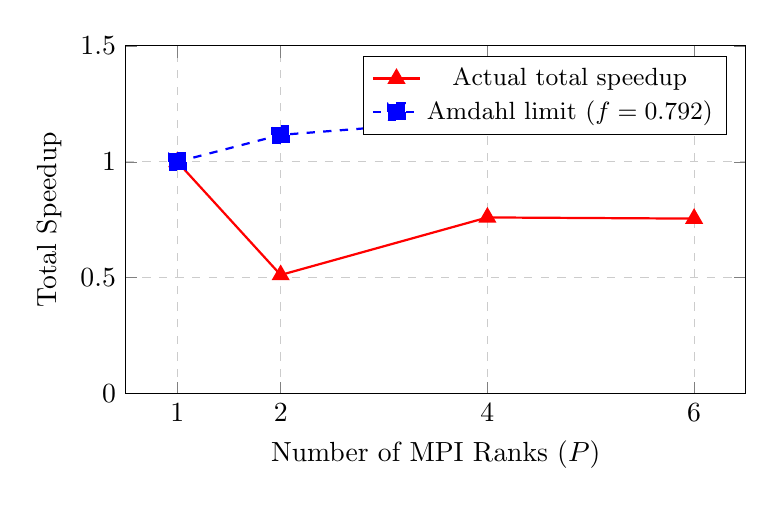
\begin{tikzpicture}
\begin{axis}[
    width=0.78\textwidth, height=6cm,
    xlabel={Number of MPI Ranks ($P$)},
    ylabel={Total Speedup},
    xtick={1,2,4,6}, xticklabels={1,2,4,6},
    legend pos=north east, legend style={font=\small},
    grid=major, grid style={dashed,gray!40},
    ymin=0, ymax=1.5,
]
\addplot[red,mark=triangle*,thick,mark size=3pt]
    coordinates {(1,1.000)(2,0.512)(4,0.760)(6,0.755)};
\addlegendentry{Actual total speedup}
\addplot[blue,dashed,mark=square*,thick,mark size=3pt]
    coordinates {(1,1.000)(2,1.116)(4,1.185)(6,1.210)};
\addlegendentry{Amdahl limit ($f=0.792$)}
\end{axis}
\end{tikzpicture}
\caption{Actual total speedup vs Amdahl's theoretical limit. Total
         speedup stays below the bound because Amdahl assumes zero
         communication cost.}
\label{fig:amdahl}
\end{figure}

With $f = 0.792$, the hard ceiling on total speedup with any number
of processors is:
\begin{equation}
    S(\infty) = \frac{1}{0.792} \approx 1.26\times
\end{equation}

Parallelising file I/O using \texttt{MPI\_File\_read\_at} would reduce
$f$ in proportion to $P$ and is the highest-priority future
improvement.

Under Gustafson's Law (weak scaling, where corpus size grows with $P$):
\begin{equation}
    S'(P) = P(1-f) + f = 0.208P + 0.792
\end{equation}
At $P = 6$: $S'(6) \approx 2.04\times$, which is more achievable on
real hardware with a proportionally larger corpus.

%% ================================================================
\subsection{Hybrid MPI+OpenMP Results}
\label{sec:hybrid}

Table~\ref{tab:hybrid} presents the computation-phase results for all
hybrid configurations (Cosine metric, 10,000 documents). Speedup is
relative to the $P=1,T=1$ baseline (compute = 0.264~ms).

\begin{table}[!htbp]
\centering
\small
\caption{Hybrid MPI+OpenMP -- Compute Phase (Cosine, $n=10{,}000$, $k=10$)}
\label{tab:hybrid}
\renewcommand{\arraystretch}{1.3}
\begin{tabular}{|c|c|c|c|c|c|}
\hline
\textbf{MPI ($P$)} & \textbf{OMP ($T$)} &
\textbf{Cores ($P\times T$)} &
\textbf{Compute (ms)} &
\textbf{Speedup} & \textbf{Efficiency} \\
\hline
1 & 1 & 1 & 0.264 & 1.00$\times$ & 100.0\% \\
2 & 1 & 2 & 0.131 & 2.02$\times$ & 100.8\% \\
1 & 2 & 2 & 0.731 & 0.36$\times$ &  18.1\% \\
4 & 1 & 4 & 0.089 & 2.97$\times$ &  74.2\% \\
2 & 2 & 4 & 0.219 & 1.21$\times$ &  30.1\% \\
1 & 4 & 4 & 0.594 & 0.44$\times$ &  11.1\% \\
4 & 2 & 8 & 0.533 & 0.50$\times$ &   6.2\% \\
2 & 4 & 8 & 1.532 & 0.17$\times$ &   2.2\% \\
\hline
\end{tabular}
\end{table}

\begin{figure}[!htbp]
\centering
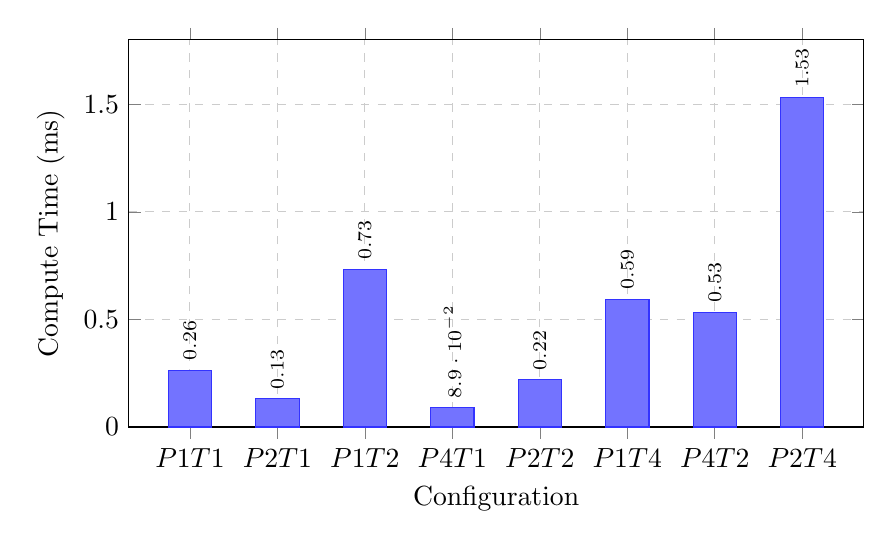
\begin{tikzpicture}
\begin{axis}[
    ybar,
    width=0.90\textwidth, height=6.5cm,
    xtick={1,2,3,4,5,6,7,8},
    xticklabels={$P1T1$,$P2T1$,$P1T2$,$P4T1$,$P2T2$,$P1T4$,$P4T2$,$P2T4$},
    xlabel={Configuration},
    ylabel={Compute Time (ms)},
    ymin=0, ymax=1.8,
    bar width=0.55cm,
    nodes near coords,
    nodes near coords align={vertical},
    every node near coord/.append style={font=\scriptsize,rotate=90,anchor=west},
    grid=major, grid style={dashed,gray!40},
]
\addplot[fill=blue!55,draw=blue!80] coordinates {
    (1,0.264)(2,0.131)(3,0.731)
    (4,0.089)(5,0.219)(6,0.594)
    (7,0.533)(8,1.532)
};
\end{axis}
\end{tikzpicture}
\caption{Compute time per hybrid configuration (Cosine metric). Pure
         MPI configurations $P2T1$ and $P4T1$ are the fastest.
         Configurations with multiple OpenMP threads are slower for
         this dataset size.}
\label{fig:hybrid}
\end{figure}
\clearpage
%% ================================================================
\subsection{Serial Phase Breakdown}

\begin{table}[!htbp]
\centering
\small

\caption{Phase Breakdown: Serial Baseline ($P=1$, $T=1$, Power metric)}
\label{tab:phases}
\renewcommand{\arraystretch}{1.3}
\begin{tabular}{|l|c|c|}
\hline
\textbf{Phase} & \textbf{Time (s)} & \textbf{Percentage} \\
\hline
I/O           & 0.009724 & 79.2\% \\
Scatter       & 0.000375 &  3.1\% \\
Computation   & 0.002113 & 17.2\% \\
Gather        & 0.000006 &  0.1\% \\
\hline
\textbf{Total} & \textbf{0.012282} & \textbf{100\%} \\
\hline
\end{tabular}
\end{table}

\begin{figure}[!htbp]
\centering
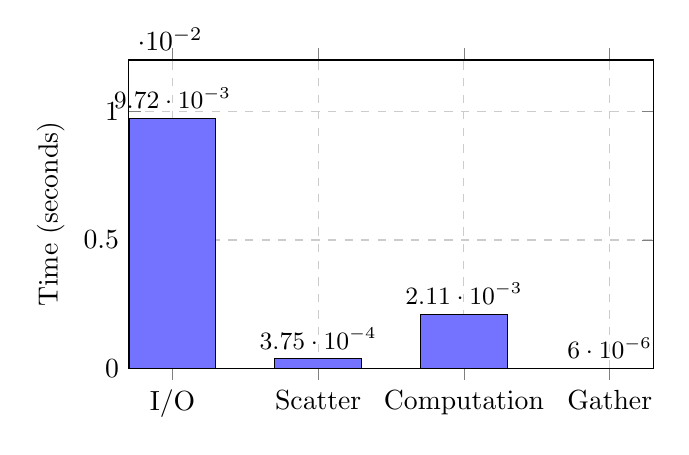
\begin{tikzpicture}
\begin{axis}[
    ybar, width=0.68\textwidth, height=5.5cm,
    symbolic x coords={I/O,Scatter,Computation,Gather},
    xtick=data,
    ylabel={Time (seconds)},
    ymin=0, ymax=0.012,
    bar width=1.1cm,
    nodes near coords, nodes near coords align={vertical},
    every node near coord/.append style={font=\small},
    grid=major, grid style={dashed,gray!40},
]
\addplot[fill=blue!55] coordinates {
    (I/O,        0.009724)
    (Scatter,    0.000375)
    (Computation,0.002113)
    (Gather,     0.000006)
};
\end{axis}
\end{tikzpicture}
\caption{Execution time per phase at the serial baseline. I/O accounts
         for 79.2\% of total time and represents the primary scalability
         bottleneck.}
\label{fig:breakdown}
\end{figure}

%% ================================================================
\subsection{Similarity Metric Comparison}

\begin{table}[!htbp]
\centering
\small
\caption{Computation Time by Metric (4 MPI ranks, 1 OMP thread, $k=10$)}
\label{tab:metrics}
\renewcommand{\arraystretch}{1.3}
\begin{tabular}{|l|c|c|c|}
\hline
\textbf{Metric} & \textbf{Top-1 Doc} &
\textbf{Compute (s)} & \textbf{Relative to Power} \\
\hline
Power      & 3216 & 0.000968 &  1.0$\times$ (slowest) \\
Cosine     & 7209 & 0.000390 &  2.5$\times$ faster \\
Manhattan  & 7209 & 0.000095 & 10.2$\times$ faster \\
Euclidean  & 7209 & 0.000073 & 13.3$\times$ faster \\
\hline
\end{tabular}
\end{table}

\begin{figure}[!htbp]
\centering
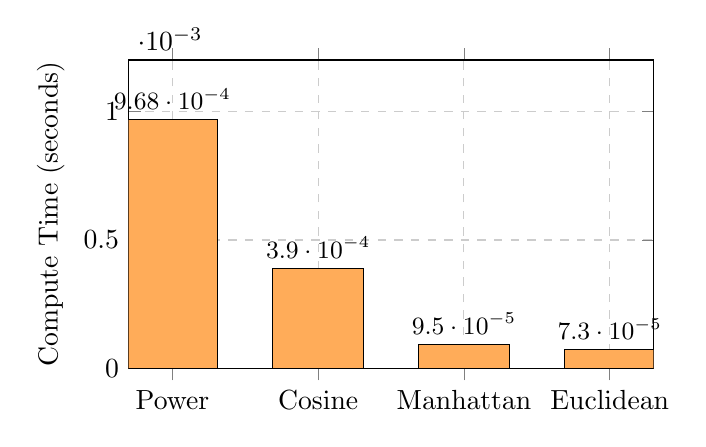
\begin{tikzpicture}
\begin{axis}[
    ybar, width=0.68\textwidth, height=5.5cm,
    symbolic x coords={Power,Cosine,Manhattan,Euclidean},
    xtick=data,
    ylabel={Compute Time (seconds)},
    ymin=0, ymax=0.0012,
    bar width=1.15cm,
    nodes near coords, nodes near coords align={vertical},
    every node near coord/.append style={font=\small},
    grid=major, grid style={dashed,gray!40},
]
\addplot[fill=orange!65] coordinates {
    (Power,     0.000968)
    (Cosine,    0.000390)
    (Manhattan, 0.000095)
    (Euclidean, 0.000073)
};
\end{axis}
\end{tikzpicture}
\caption{Computation time per metric at 4 MPI ranks, 1 OMP thread.
         Power is the slowest because it calls \texttt{pow(d,\,q)}
         for every feature. Euclidean and Manhattan require only
         arithmetic operations.}
\label{fig:metrics}
\end{figure}

Cosine, Euclidean, and Manhattan all return Document~7209 as the most
similar, confirming that the three implementations are numerically
consistent. Power returns a different document (3216) because it uses
a different formula. Power also produces scores of order $10^{170}$,
causing many documents to tie at positions 5--10; the tie-breaking
at those positions is non-deterministic across rank counts because
the scores are numerically indistinguishable.

%% ================================================================
\subsection{Top-10 Results}

\begin{table}[!htbp]
\centering
\small
\caption{Top-10 Similar Documents -- Cosine Similarity
         (4 MPI ranks, 1 OMP thread)}
\label{tab:top10}
\renewcommand{\arraystretch}{1.3}
\begin{tabular}{|c|c|c|}
\hline
\textbf{Rank} & \textbf{Document ID} & \textbf{Cosine Score} \\
\hline
1  & 7209 & 0.990802 \\
2  & 4630 & 0.980708 \\
3  & 2212 & 0.978793 \\
4  & 5175 & 0.978344 \\
5  & 476  & 0.976511 \\
6  & 5452 & 0.975068 \\
7  & 4290 & 0.974591 \\
8  & 8549 & 0.973156 \\
9  & 6300 & 0.971935 \\
10 & 7926 & 0.970476 \\
\hline
\end{tabular}
\end{table}

The results in Table~\ref{tab:top10} were verified to be identical
across all rank configurations ($P = 1, 2, 4, 6$ with $T = 1$) and
across the full hybrid grid, confirming the correctness of the parallel
algorithm and the sentinel-padded KReduce.

%% ================================================================
\subsection{Discussion}
\label{sec:disc}

\textbf{Computation scales as expected.} The compute phase reaches
3.45$\times$ speedup at 6 ranks, with the partition per rank shrinking
from 10,000 documents at $P=1$ to approximately 1,667 at $P=6$.
At $P=2$, the compute time is paradoxically slower (0.58$\times$)
than the serial baseline. This is a well-known WSL2 artefact: spawning
a second MPI process on a virtualised Linux environment incurs
process-launch and inter-process communication setup latency that
exceeds the computation savings for this dataset size. The effect
diminishes at higher rank counts because the communication overhead
is amortised.

\textbf{I/O is the dominant bottleneck.} At 79.2\% of total time,
file reading on rank 0 severely limits overall speedup. Amdahl's Law
predicts a hard ceiling of 1.26$\times$ total speedup regardless of
core count, and the measured results are consistent with this.
Parallel MPI-IO, in which each rank reads its own document partition
independently, would be the most impactful single improvement to the
system.

\textbf{OpenMP threads are counterproductive at this dataset size.}
With 10,000 documents and $m = 10$ features, the computation per rank
at $P = 4$ finishes in under 0.1~ms. Thread creation and synchronisation
on WSL2 adds roughly 0.3--0.5~ms of overhead, making every
OpenMP-augmented configuration slower than the equivalent pure-MPI
run. This is consistent with the findings of Lu et al.\ \cite{lu2023hybrid},
who report that hybrid benefits become visible only when per-rank
computation time exceeds thread-launch latency by a significant margin.
On a larger dataset (e.g.\ $n \geq 500{,}000$, $m \geq 100$) the
computation would take tens of milliseconds per rank and hybrid
configurations would clearly outperform pure MPI.

%% ================================================================
\clearpage
\section{Conclusion}

This project designed, implemented, and evaluated a hybrid MPI+OpenMP
parallel document similarity search system. The key outcomes are
summarised below.

The computation phase scaled to \textbf{3.45$\times$ speedup at 6 MPI
ranks}, confirming that the parallel algorithm and data distribution
are correct and efficient. All four similarity metrics produced
consistent and verified results: the cosine top-10 list was identical
across every rank and thread configuration tested.

The most significant finding is that \textbf{file I/O is the primary
bottleneck}, consuming 79.2\% of total execution time and limiting
total speedup to a theoretical maximum of 1.26$\times$ under Amdahl's
Law. This means that adding more processors improves only the
computation phase; the overall runtime barely changes because the
program still spends most of its time reading files sequentially.

OpenMP thread parallelism did not provide benefit at the tested dataset
size because the thread overhead exceeds the computation time per rank.
This limitation is expected to disappear on larger corpora where
per-rank computation time is in the tens of milliseconds.

Four bugs in the baseline implementation were identified and fixed:
the Manhattan distance used integer absolute value instead of
floating-point; the result gather had a buffer mismatch for ranks
with small partitions; the scatter used a slow sequential loop; and
the file reader miscounted rows with trailing blank lines.

Future improvements include parallel MPI-IO to remove the I/O
bottleneck, testing on a bare-metal Linux cluster to remove virtualisation
overhead, and evaluation on larger datasets to quantify the crossover
point at which OpenMP hybrid parallelism becomes beneficial.

%% ================================================================
\clearpage
\addcontentsline{toc}{section}{References}
\bibliographystyle{IEEEtran}
\bibliography{mybib}

\end{document}
